\section{Minimalizacja w 1-D}
  \begin{frame}{Minimalizacja w 1-D}
    \begin{block}{Przydatność metod 1-D dla zag. n-D}
      \begin{itemize}
        \item Prosta ilustracja ogólnych problemów
        \item Metody 1-D są często elementem składowym metod n-D

      \end{itemize}

    \end{block}

  \end{frame}

\subsection{Przeglądanie siatki (grid search)}
  \begin{frame}{Przeglądanie siatki \emph{(grid search)}}
    \begin{block}{Realizacja}
      \begin{itemize}
        \item Przegląd wszystkich elementów iloczynu kartezjańskiego podzbiorów parametrów.
        \item Wybór wartości najmniejszej.
      \end{itemize}
    \end{block}

    \begin{block}{Zalety}
      \begin{itemize}
        \item Absolutna prostota, problem typu embarrassingly parallel.
        \item Bezwzględna zbieżność.
        \item Brak "czułości" na szczegółowe zachowanie się $F(x)$.
      \end{itemize}
    \end{block}

    \begin{block}{Wady}
      \begin{itemize}
        \item Nie może być stosowana dla przedziału nieskończonego.
        \item Nieefektywna, nie "uczy się" własności funkcji.
      \end{itemize}
    \end{block}
  \end{frame}

  \begin{frame}{Przeglądanie siatki \emph{(grid search)}}
    Problem z doborem rozmiaru siatki, tak aby nie zgubić szukanej wartości.

    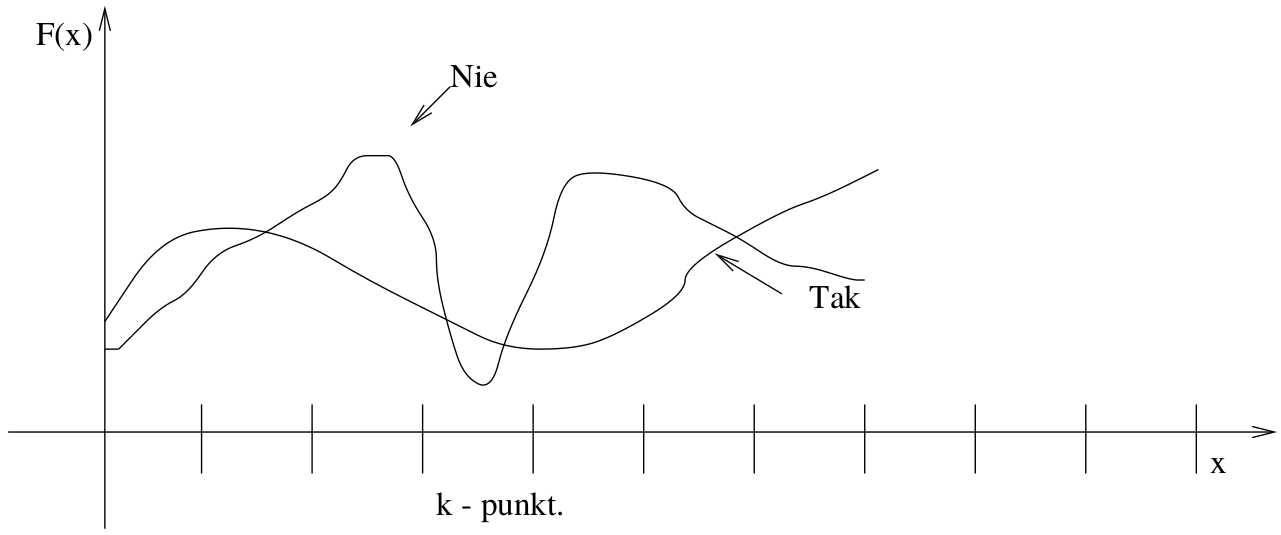
\includegraphics[width=1\textwidth]{img/17/przegladanie_siatki}
  \end{frame}

  \begin{frame}{Przeglądanie siatki \emph{(grid search)}}
    \textbf{Założenie:} Poszukujemy minimum w k-D dysponując k zbiorami parametrów po 10 000 elementów każdy.

    \begin{tabular}{@{} c l c c c @{}}
      & $ 100 $ & punktów & w & 1 -- D \\
      $ $ Zawężamy obszar do 1\% $ \Rightarrow $ & $ 100^{2} $ & & w & 2 -- D \\
      & $ 100^{10} $ & & w & 10 -- D \\
    \end{tabular}

    Przy czasie obliczeń jednej wartości $F(x) \approx 10^{-5}s$
    \begin{displaymath}
      \text{Czas obliczeń: } t_o = \frac{10^{20}*10^{-5}s}{\underbrace{\pi * 10^{7}}_{\text{sek. w roku}}} \approx 3 * 10^{7}lat \text{!}
    \end{displaymath}
    \begin{flushright}
      \emph{Zadanie:} porównaj $\to$ całki w n-D
    \end{flushright}
  \end{frame}

\subsection{Metoda złotego podziału (golden section search)}
    \begin{frame}{Metoda złotego podziału \emph{(golden section search)}}
    \begin{block}{Definicja funkcji unimodalnej}
      Funkcję $f(x)$ nazywamy \emph{unimodalną} na przedziale
      $[a{,}b]$ jeżeli:
      \begin{enumerate}
        \item $\exists x^{*}\in [a{,}b] : f(x^{*}) = min_{x \in [a{,}b]}f(x)$
        \item $\forall x_{1}{,}x_{2} : a \leq x_{1} < x_{2} \leq b$ zachodzi:
        \begin{itemize}
          \item $x_{2} \leq x_{*} \Rightarrow f(x_{1}) > f(x_{2})$
          \item $x_{1} \geq x_{*} \Rightarrow f(x_{1}) < f(x_{2})$
        \end{itemize}
      \end{enumerate}
    \end{block}
    \begin{block}{Założenia}
      \textbf{Dane:} $f$ -- funkcja unimodalna na przedziale $[a, b]$\\
      \textbf{Szukane:} minimum $x_0$ funkcji $f$ na przedziale $[a, b]$
    \end{block}
  \end{frame}

  \begin{frame}{Metoda złotego podziału \emph{(golden section search)}}
    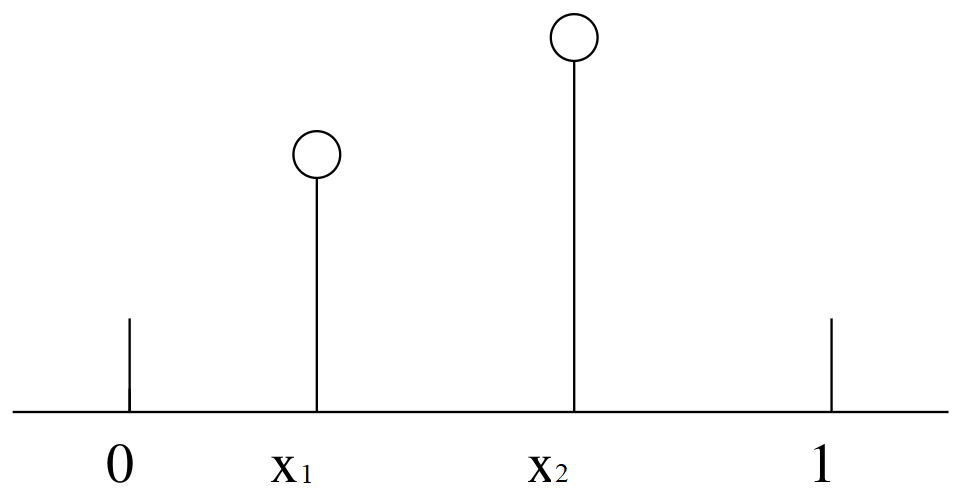
\includegraphics[width=0.9\textwidth]{img/17/f_unimodalna}
    \\
    $F(x)$ - f. unimodalna
  \end{frame}

  \begin{frame}{Metoda złotego podziału \emph{(golden section search)}}
    \begin{block}{Realizacja}
      $r$ -- współczynnik redukcji po każdym etapie
      \begin{enumerate}
        \item Obliczamy nową długość przedziałów $ d = \frac{1}{r}(b - a) $
        \item $ x_L = b - d, x_R = a + d $
        \item Jeżeli $ f(x_L) > f(x_R) \Rightarrow x_0 \in [x_L, b] $,
              $ a := x_L \text{, } $\\
              Jeżeli $ f(x_L) < f(x_R) \Rightarrow x_0 \in [a, x_R] $,
              $ b := x_R \text{, } $
        \item Procedurę powtarzamy, aż do osiągnięcia żądanej zbieżności.
      \end{enumerate}
    \end{block}
    \begin{block}{Minimalizacja ewaluacji}
      \textbf{Problem:} Chcemy zminimalizować liczbę ewaluacji funkcji $f$.\\
      \textbf{Rozwiązanie:} Dobieramy współczynnik $r$, aby w kolejnym kroku wykorzystać jedną z dwóch próbek: $f(x_L)$ lub $f(x_R)$.
    \end{block}
  \end{frame}
  \begin{frame}{Metoda złotego podziału \emph{(golden section search)}}
    $t$ -- współczynnik redukcji po każdym etapie\\
    Rozmieszczenie punktów:\\
    Dla $[0, 1]$ -- długość przedziału po pierwszym etapie: $d_1 = t$\\
    \centering
    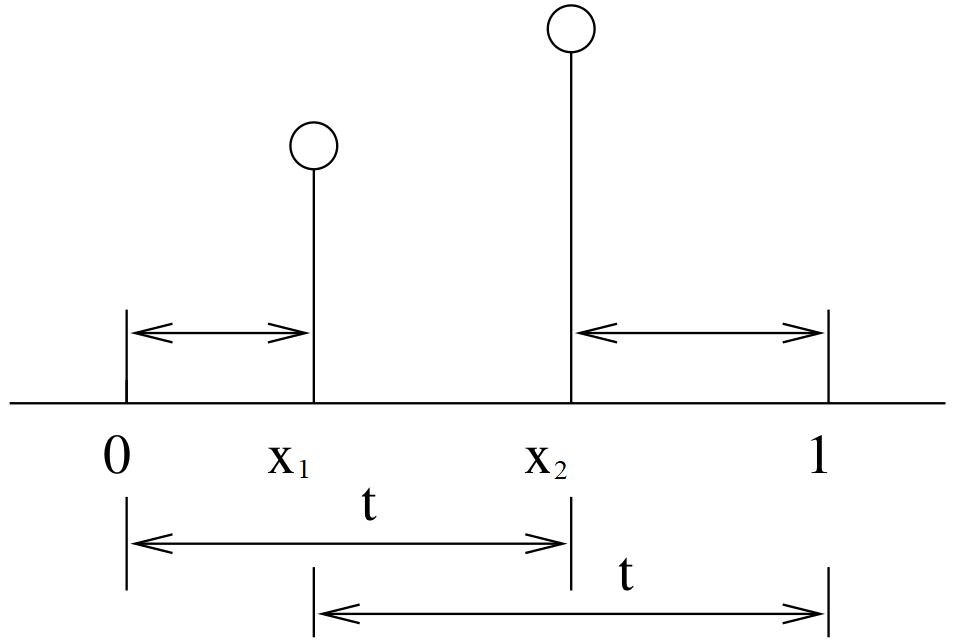
\includegraphics[height=0.6\textheight]{img/17/f_uni2}
  \end{frame}

  \begin{frame}{Metoda złotego podziału \emph{(golden section search)}}
    Po wyznaczeniu $f(x_3) \to$ długość przedziału -- $t^{2}$
    \begin{displaymath}
      t^{2} = 1 - t \Rightarrow t = \frac{\sqrt{5} - 1}{2} \approx 0,616 \to \text{\emph{złoty podział}}
    \end{displaymath}
    Dla zadanej liczby kroków -- optymalna.\\
    Podobna metoda dla zbiorów -- Fibonacci search technique.
    \centering
    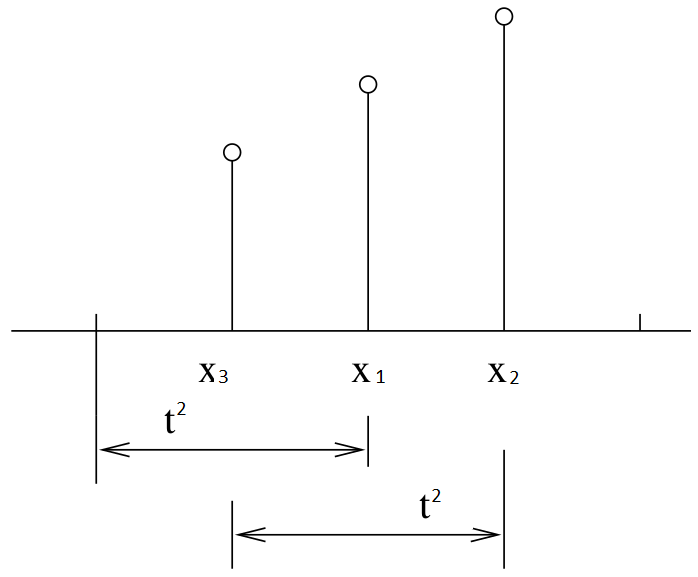
\includegraphics[height=0.55\textheight]{img/17/fibb}
  \end{frame}

  \begin{frame}{Metoda złotego podziału \emph{(golden section search)}}
    \begin{block}{Optymalność}
      Metoda minimax -- minimalizuje maksymalną liczbę określeń
      $f(x)$.
    \end{block}
    \begin{block}{Optymalność pesymistyczna}
      Odpowiednik najlepszej strategii w grze przeciwko
      inteligentnemu przeciwnikowi.\\
      Podejście dobre dla patologicznych funkcji.
    \end{block}
    \begin{examples}{Modyfikacje metody -- Przykład}
      \textbf{Metoda Bermana}
      $x_{0} = \frac{a + b}{2}$; poszukiwanie tam, gdzie $f$ maleje.
      Ustalony krok, w drugą stronę -- z mniejszym krokiem.
    \end{examples}
  \end{frame}

\subsection{Kwadratowa interpolacja i aproksymacja}
  \begin{frame}{Kwadratowa interpolacja i aproksymacja}
    \begin{block}{Założenia}
      Wykres funkcji $f(x)$ jest parabolą.
    \end{block}
    \begin{block}{Realizacja}
      \begin{itemize}
        \item Interpolujemy $f(x)$ funkcją kwadratową w 3 punktach: $x_{1}{, }x_{2}{, }x_{3}$.
        \item Min $f(x) $ to min paraboli przechodzącej przez
        $x_{1}{, }x_{2}{, }x_{3}$, znajduje się w punkcie $x_4$:
        \begin{displaymath}
          x_4 = - \frac{
            \frac{f_{1}*(x_{2}+x_{3})}{(x_{1}-x_{2})*(x_{1}-x_{3})} +
            \frac{f_{2}*(x_{1}+x_{3})}{(x_{2}-x_{1})*(x_{2}-x_{3})} +
            \frac{f_{3}*(x_{1}+x_{2})}{(x_{3}-x_{1})*(x_{3}-x_{2})}
          }{2 * \left[
            \frac{f_{1}}{(x_{1}-x_{2})*(x_{1}-x_{3})} +
            \frac{f_{2}}{(x_{2}-x_{1})*(x_{2}-x_{3})} +
            \frac{f_{3}}{(x_{3}-x_{1})*(x_{3}-x_{2})}
          \right]}
        \end{displaymath}
        \begin{flushright}
          \emph{Zadanie:} Sprawdzić ten wzór.
        \end{flushright}
      \end{itemize}
    \end{block}
  \end{frame}

  \begin{frame}{Kwadratowa interpolacja i aproksymacja}
    \begin{block}{Realizacja cd.}
      \begin{itemize}
        \item $x_{4}$ -- zastępuje jeden z $x_{1}{,}x_{2}{,}x_{3}$,
        wyznaczamy nowy $ x_{4} $.
        \item Procedurę kończymy gdy wartość $f(x_{4})$ jest bliska $f(x_{3})$\\
        z zadaną dokładnością.
      \end{itemize}
    \end{block}
    \begin{block}{Problemy}
      \begin{enumerate}
        \item Na każdym kroku $x_{1}{,}x_{2}{,}x_{3}$ mogą
        wyznaczać $max$, a nie $min$ powodując rozbieżność.
        \item Gdy $x_{1}{,}x_{2}{,}x_{3}$ leżą prawie na prostej, otrzymujemy duży krok:
        \begin{itemize}
          \item Trudności numeryczne
          \item Rozbieżność
        \end{itemize}
        \item Który z poprzednich punktów odrzucić?
        \item Możliwe oscylacje wokół minimum, zamiast zbieżności.
      \end{enumerate}
    \end{block}
  \end{frame}

    \begin{frame}{Kwadratowa interpolacja i aproksymacja}
      \begin{block}{Możliwe zabezpieczenia}
        Zaniechanie metody przy wystąpieniu trudności.
      \end{block}
      \begin{block}{Zastosowanie}
        W ostatniej fazie minimalizacji funkcji $f$.\\
        (Funkcje fizyczne są zwykle paraboliczne w pobliżu minimum.)
      \end{block}
    \end{frame}

\subsection{Metoda prób i błędów (success-failure method)}
  \begin{frame}{Metoda prób i błędów \emph{(success-failure method)}}
    \begin{block}{Założenie}
      Procedura składa się z dwóch części:
      \begin{itemize}
        \item Iteracyjne zawężenie przedziału -- podobne do grid search.
        \item Kwadratowa interpolacja na otrzymanym przedziale.
      \end{itemize}
    \end{block}
    $x_{0}$ -- start point, $d$ -- initial step size
    \begin{itemize}
      \item Gdy $f(x_{0} + d) < f(x_{0}) $ -- sukces:\\
      $x_{0} \to x_{0} + d,$ \\
      $d \to \alpha * d, \alpha$ -- expansion factor
      $(\alpha > 1)$
      \item Gdy $f(x_{0} + d) > f(x_{0}) $ -- niepowodzenie: \\
      $d \to -\beta * d, \beta$ -- contraction factor
      $(\beta < 1)$
    \end{itemize}
    $\alpha$ oraz $\beta$ -- ustalamy arbitralnie\\
    Procedurę powtarzamy do zbieżności, tj. $|f(x_{0} + d) - f(x_{0})| < \epsilon$.
  \end{frame}

  \begin{frame}{Metoda prób i błędów \emph{(success-failure method)}}
    Minimum jest zawężone (bracketed), wtedy mamy trzy punkty typu:\\
    \begin{center}
      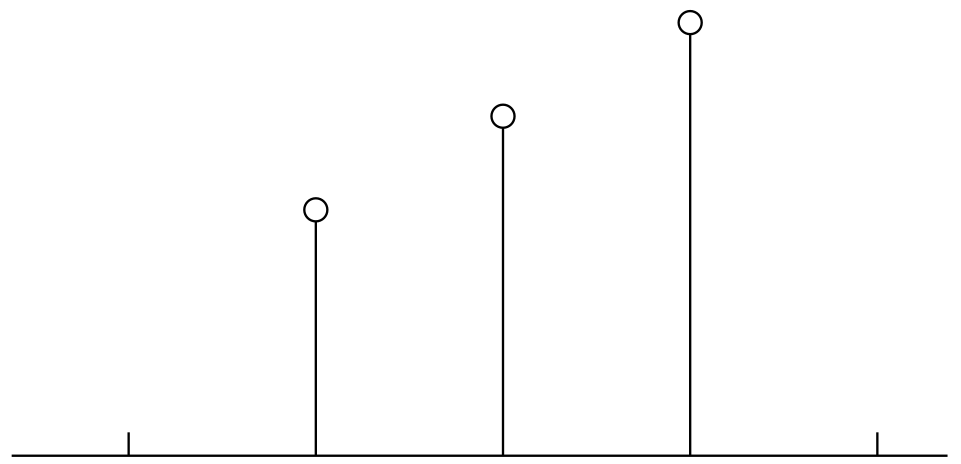
\includegraphics[width=0.7\textwidth]{img/17/s-f}
    \end{center}
    Są one \emph{punktem startowym} interpolacji kwadratowej.\\
    \textbf{Uniwersalna, efektywna metoda 1-D dla ogólnych funkcji.}
  \end{frame}
